\documentclass[11pt]{article}

\usepackage[margin=1in]{geometry}
\usepackage{booktabs}
\usepackage{graphicx}
\usepackage{listings}
\usepackage{xcolor}
\usepackage[hidelinks]{hyperref}

\lstset{basicstyle=\ttfamily\small, columns=fullflexible, breaklines=true,
        frame=single, xleftmargin=1em}

\newcommand{\OaInstr}{28}
\newcommand{\OcInstr}{21}
\newcommand{\OaDram}{339}
\newcommand{\ObDram}{176}
\newcommand{\OaCycles}{23421}
\newcommand{\OcCycles}{12710}
\newcommand{\LlvmTag}{llvmorg-22.1.8}
\newcommand{\GitSha}{4fda49447503}
\newcommand{\BestPass}{\texttt{npu-fuse-ops}}
\newcommand{\BestPassCycles}{298}
\newcommand{\BestPassInstrs}{4}
\newcommand{\BestPassTightCycles}{-96}
\newcommand{\BestPassTightDram}{-6.1}


\title{An MLIR Backend for a Simulated Edge NPU}
\author{Olajide Badejo}
\date{\today}

\begin{document}
\maketitle

\begin{abstract}
This report describes a from scratch MLIR compiler backend that takes a trained
ONNX model to an executable instruction stream for a simulated, simplified edge
NPU, together with a C++ simulator that runs the stream and reports numerical
correctness against onnxruntime and simulated performance from an analytical cost
model. The compiler uses two dialects: a tensor level dialect for optimization and
an instruction level dialect with an explicit two level memory model. It performs
canonicalization, constant folding, a dedicated BatchNorm folding pass, operator
fusion, and dead code elimination, then lowers to the instruction level through
the dialect conversion framework, allocates a fixed size scratchpad with spills to
DRAM, and encodes a documented binary format. Every performance number here is a
simulated estimate, not a measurement.
\end{abstract}

\section{Introduction}

Edge inference accelerators are simple compared with general purpose processors.
They run static neural network graphs, keep data in a small fast scratchpad, and
move it to and from DRAM under explicit control. Building a compiler for such a
target is a good way to learn how a real machine learning compiler is organized,
because the interesting problems (memory placement, operator fusion, a documented
instruction encoding, and validation against a reference) all appear in a
tractable form.

This project is a from scratch MLIR backend for a simulated edge NPU. It takes a
trained ONNX model and lowers it, through two custom dialects, to an executable
instruction stream, which a C++ simulator runs to produce both the numerical
result and an analytical performance estimate. The compiler is built as a small
out of tree MLIR project linked against a prebuilt LLVM and MLIR at a pinned tag.

Two commitments shape the work. First, correctness is validated end to end against
onnxruntime within stated tolerances, so the compiler is not merely plausible but
demonstrably right on the test models. Second, every performance number is an
analytical estimate from a documented cost model and is labeled a simulated
estimate throughout, never presented as a measurement.

\section{Related work}

MLIR provides the reusable compiler infrastructure this project builds on, in
particular the dialect mechanism, the operation definition specification in
TableGen, and the dialect conversion framework used for the representation
changing lowering \cite{mlir2021}. Deep learning compilers such as TVM established
the pattern of importing a framework graph, optimizing it, and lowering it to a
hardware target \cite{tvm2018}. The hardware model here is a small systolic array
with a two level memory, the design point studied at scale by the Tensor
Processing Unit \cite{tpu2017} and analyzed as a dataflow problem by Eyeriss
\cite{eyeriss2016}, whose emphasis on minimizing data movement motivates the
scratchpad and fusion work in this compiler.

The frontend consumes ONNX \cite{onnx}, the interchange format that trained models
are exported to. The two dialect structure, a tensor level dialect for
optimization and an instruction level dialect after memory placement, mirrors the
approach taken by production MLIR backends such as Tenstorrent's tt-mlir
\cite{ttmlir}.

\section{Architecture}

The pipeline is a sequence of well defined stages. A Python importer reads the
ONNX model and, using the MLIR Python bindings, builds \texttt{npu} dialect IR, a
tensor level representation whose values conceptually live in DRAM. A sequence of
passes optimizes this IR to a fixed point. The dialect conversion framework then
lowers it to the \texttt{npuisa} dialect, an instruction level representation in
which values are scratchpad resident buffers and data crosses the DRAM boundary
only through explicit DMA. A scratchpad allocator assigns each buffer a byte
offset and spills to DRAM when the working set exceeds the budget. The instruction
encoder serializes the result to a documented binary format, which a disassembler
can render and which the simulator executes.

The compiler is a small out of tree CMake project. It never builds LLVM itself; it
links against a prebuilt LLVM and MLIR at a pinned release tag. This keeps the
per change build in the seconds to minutes range after the one time toolchain
build. The driver, \texttt{npu-compile}, wraps the whole pipeline with
optimization levels and staged output so any intermediate can be inspected.

\section{Dialect design}

The \texttt{npu} dialect is the tensor level. Values are builtin ranked fp32
tensors, which keeps interoperability with the MLIR infrastructure so that generic
folding and dead code elimination apply without op specific support. Convolution
and matmul take an optional bias operand and carry a fused activation attribute
rather than exploding into a family of named fused ops. This mirrors the fused
operator style of TFLite and gives the fusion pass a single clean target. Every op
that computes a pure function of its operands carries the \texttt{Pure} trait, and
each op with shape or type constraints has an ODS verifier. The dialect reference
is generated from the op definitions so it cannot drift.

The \texttt{npuisa} dialect is the instruction level, after memory placement. A
value of \texttt{!npuisa.buffer} type is a scratchpad resident tensor. DRAM
tensors move to and from the scratchpad through \texttt{dma\_load} and
\texttt{dma\_store}, and compute instructions read and write buffers only. The
instruction stream is straight line, since inference graphs are static DAGs, so
the instruction set has no branches. Each buffer producing instruction carries an
address attribute that the allocator fills in.

\section{Optimization passes}

Canonicalization and constant folding run through the built in greedy driver,
using the folders and canonicalization patterns attached to the ops. Constant
subgraphs collapse to a single constant, and structural patterns such as relu
idempotence and reshape of reshape fire.

The BatchNorm folding pass is dedicated and does real tensor arithmetic at compile
time. At inference the scale, offset, mean, and variance of a batch normalization
are constants, so a batch norm following a convolution with no activation between
them is exactly another convolution with rescaled weights and bias:
\[
  \mathrm{coef}[o] = \frac{\mathrm{scale}[o]}{\sqrt{\mathrm{var}[o] + \epsilon}},
  \quad W'[o] = W[o]\,\mathrm{coef}[o],
  \quad b'[o] = \mathrm{coef}[o]\,(b[o] - \mathrm{mean}[o]) + \mathrm{offset}[o].
\]
The pass matches this pattern, computes the new constant tensors, and emits a
single convolution.

Operator fusion folds a trailing relu into a producing convolution or matmul by
setting the fused activation attribute. Because those ops already carry the bias
as an operand, the result is a single fused convolution or matmul that computes
the linear operation, the bias, and the activation together. The intermediate
therefore stays in the scratchpad rather than being written to DRAM and read back.

Dead code elimination needs no custom pass. Because every op is \texttt{Pure}, the
canonicalizer removes unused ops and \texttt{symbol-dce} removes unused private
functions. The three optimization levels compose these: \texttt{-O0} imports and
verifies, \texttt{-O1} adds canonicalization and folding, and \texttt{-O2} adds
fusion and dead code elimination.

\section{ONNX frontend}

The frontend runs \texttt{onnx.checker} and shape inference before importing, so a
malformed model is rejected up front and every intermediate tensor has a static
shape. It then walks the graph in topological order, turning initializers into
constants and each node into the matching \texttt{npu} op. The supported opset 17
subset covers convolution, Gemm, matmul, elementwise add, relu, max and average
pooling, batch normalization, reshape, and flatten. A Gemm with a transposed
weight folds the transpose into the constant at import time so the plain matmul is
correct. Anything outside the supported set fails loudly with the op name, never
emitting silently wrong IR.

The test models are generated, never downloaded, from small seeded PyTorch
networks exported with \texttt{torch.onnx.export}, so the suite is fully self
contained and reproducible from the seed. The core model is a LeNet style
convolutional network.

\section{ISA and simulator}

The instruction set has a two level memory model: DRAM holds inputs, constants,
and outputs; the scratchpad, a small fixed size fast memory with a default of one
megabyte, holds the working set. The opcodes are NOP, HALT, DMA\_LOAD, DMA\_STORE,
CONV2D, MATMUL, RELU, ADD, MUL, POOL\_MAX, POOL\_AVG, and RESHAPE. The binary
format is a fixed header followed by tagged, length prefixed records, which is
simpler to get right and to disassemble than a bit packed encoding while remaining
a real, documented format. The \texttt{npu-objdump} tool renders the DRAM layout
and the instruction stream.

The simulator executes the stream against DRAM and scratchpad arrays with fp32
kernels for each instruction. Its cost model is analytical, not cycle accurate.
DMA costs bytes over an assumed bandwidth; convolution and matmul cost their
multiply accumulate count over an assumed systolic throughput of 256 operations
per cycle, the arithmetic of a sixteen by sixteen array; elementwise instructions
cost their element count over a lane width; and every instruction charges a fixed
issue overhead. These constants are documented assumptions, and the cycle and DRAM
figures the simulator reports are simulated estimates.

\section{Evaluation}

Correctness is validated end to end. The compiled and simulated output of the
LeNet model is compared against \texttt{onnxruntime} on a seeded random input; the
maximum absolute difference is at the level of fp32 rounding, on the order of
$10^{-8}$, at every optimization level and both under a generous budget and under
a tight budget that forces spilling. The benchmark harness records one result per
cell, each carrying a manifest of the git revision, the LLVM tag \LlvmTag, the
tool versions, and the cost model constants, so every number below traces to a
recorded experiment. Table~\ref{tab:results} is generated from those files.

\begin{table}[h]
  \centering
  \begin{tabular}{llrrrrr}
\toprule
Model & O & Budget (KB) & Instrs & Cycles & DRAM (KB) & Max error \\
\midrule
lenet & 0 & 140 & 91 & 23421 & 339.3 & 3.0e-08 \\
lenet & 1 & 140 & 94 & 33834 & 502.0 & 3.0e-08 \\
lenet & 2 & 140 & 86 & 33930 & 508.1 & 3.0e-08 \\
lenet & 0 & 1024 & 91 & 23421 & 339.3 & 3.0e-08 \\
lenet & 1 & 1024 & 82 & 13008 & 176.6 & 3.0e-08 \\
lenet & 2 & 1024 & 70 & 12710 & 176.6 & 3.0e-08 \\
\bottomrule
\end{tabular}

  \caption{Per cell results: instruction count, simulated cycles, total DRAM
    traffic, and maximum absolute error against onnxruntime. Cycle and DRAM
    figures are simulated estimates.}
  \label{tab:results}
\end{table}

\begin{figure}[h]
  \centering
  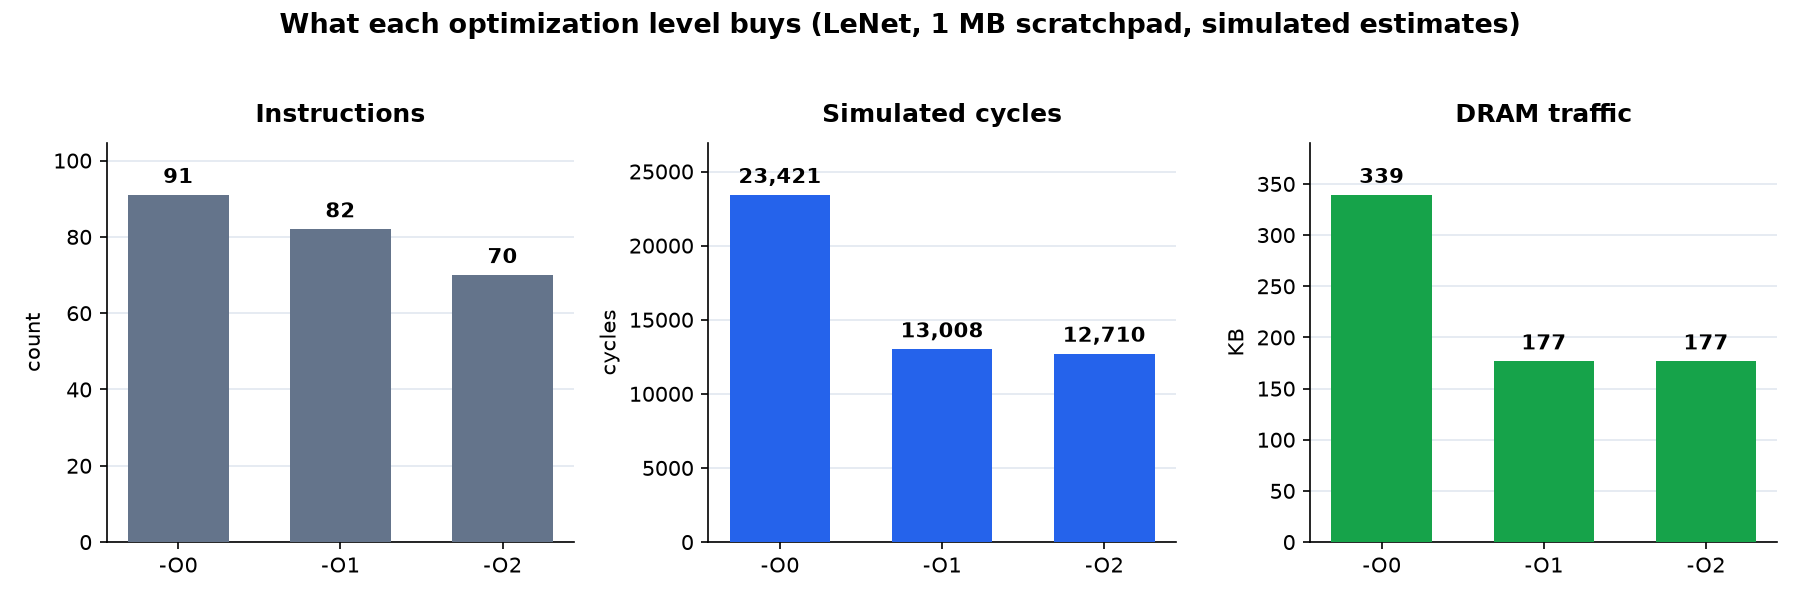
\includegraphics[width=\textwidth]{../docs/images/optimization_levels}
  \caption{What each optimization level buys on LeNet at the one megabyte budget:
    instruction count, simulated cycles, and DRAM traffic all fall from
    \texttt{-O0} to \texttt{-O2}, while the numerics stay exact. Simulated
    estimates.}
  \label{fig:levels}
\end{figure}

Two effects stand out at the one megabyte budget, where nothing spills. Moving
from \texttt{-O0} to \texttt{-O1}, canonicalization and dead code elimination
remove the transposed Gemm weight constants that the importer leaves behind, and
the total DRAM traffic falls from \OaDram{} KB to \ObDram{} KB. Moving to
\texttt{-O2}, fusion folds the four activations into their producers, and the
instruction count falls from \OaInstr{} to \OcInstr{} while the simulated cycles
fall from \OaCycles{} to \OcCycles{}.

\subsection{What each pass buys, one at a time}

The level comparison above says what \texttt{-O2} buys over \texttt{-O0}. It
cannot say what any single pass buys, because the levels are cumulative. Table
\ref{tab:ablation} answers that directly: each row is the full \texttt{-O2}
pipeline with one pass removed, compiled, encoded, simulated, and checked
against onnxruntime exactly as a normal cell is. The deltas are ablated minus
full \texttt{-O2}, so a positive number is what removing the pass costs, which
is the pass earning its place.

\begin{table}[h]
  \centering
  \begin{tabular}{llrrrrr}
\toprule
Budget & Pass removed & Instrs & $\Delta$ & Cycles & $\Delta$ & $\Delta$ DRAM (KB) \\
\midrule
1024 KB & \texttt{canonicalize} & 21 & +0 & 12710 & +0 & +0.0 \\
1024 KB & \texttt{npu-fuse-ops} & 25 & +4 & 13008 & +298 & +0.0 \\
1024 KB & \texttt{symbol-dce} & 21 & +0 & 12710 & +0 & +0.0 \\
140 KB & \texttt{canonicalize} & 29 & +0 & 33930 & +0 & +0.0 \\
140 KB & \texttt{npu-fuse-ops} & 31 & +2 & 33834 & -96 & -6.1 \\
140 KB & \texttt{symbol-dce} & 29 & +0 & 33930 & +0 & +0.0 \\
\bottomrule
\end{tabular}

  \caption{Leave one out ablation of every \texttt{-O2} pass, at both scratchpad
  budgets. Instructions, cycles, and DRAM are simulated estimates from the
  analytical cost model, not measurements. Deltas are the ablated pipeline minus
  full \texttt{-O2} at the same budget, so a positive delta means removing the
  pass made the program worse. \texttt{canonicalize} is ablated everywhere it
  appears, which is twice in the \texttt{-O2} pipeline.}
  \label{tab:ablation}
\end{table}

At the generous budget only one pass buys anything: \BestPass{} is worth
\BestPassCycles{} simulated cycles and \BestPassInstrs{} instructions, and
removing either \texttt{canonicalize} or \texttt{symbol-dce} produces a byte
identical program. That is not a measurement error. \texttt{-npu-fuse-ops}
drives its patterns with a greedy rewriter whose fixed point loop folds
constants and removes dead operations as a side effect, so on this model it
subsumes everything canonicalization had to contribute. Canonicalization still
matters at \texttt{-O1}, where it is the only pass and is responsible for the
whole drop from \OaDram{} KB to \ObDram{} KB; it is redundant only in the
presence of fusion. This is exactly the interaction a leave one out ablation
exposes and a per pass measurement cannot, since measured in isolation
canonicalization does remove operations.

The tight budget reverses the sign. Removing \BestPass{} there changes the
simulated cycles by \BestPassTightCycles{} and the DRAM traffic by
\BestPassTightDram{} KB, both of which are improvements: fusion makes the
program worse when the scratchpad cannot hold the working set. Fusing an
activation into its producer extends that value's live range, and under a budget
that already forces spilling, a longer live range costs a spill and its reload.
A table reporting only the generous budget would have shown fusion as the one
pass worth having and missed that it is counterproductive under pressure.

The tight budget rows show the memory model at work. When the scratchpad cannot
hold the working set, the allocator spills buffers to DRAM and reloads them, which
raises the instruction count and the DRAM traffic relative to the generous budget.
The numerics are unchanged, because a spill is a value preserving round trip.
Finding and fixing a bug in that round trip, where spill temporaries were not
being given distinct DRAM addresses, is one of the cases the benchmark suite
caught and the debug report discusses.

\section{Conclusion}

The result is a working MLIR backend that takes a trained ONNX model to an
executable instruction stream for a simulated edge NPU and runs it with validated
numerics. The two dialect structure keeps the tensor level optimizations separate
from the instruction level memory model, the dialect conversion framework makes
the lowering a principled representation change rather than an ad hoc rewrite, and
the benchmark suite ties every reported number to a recorded experiment.

The natural next steps are INT8 quantization, which the dialect and cost model were
designed to accommodate, and a wider set of test models to exercise the depthwise
and concatenation paths. The debug report, a companion to this document, records
the problems met along the way and how they were resolved.


\bibliographystyle{plain}
\bibliography{references}

\end{document}
